\documentclass{article}
\usepackage[utf8]{inputenc}

\title{Arbol de Decisión}
\author{Valeria Ybarra López}
\date{29, Marzo 2025}
\usepackage [latin1]{inputenc}
\usepackage{xcolor} 
\usepackage{graphicx}
\usepackage{listings}
\usepackage{amsmath}
\usepackage{float}
\usepackage{graphics}
\usepackage{graphicx}
\usepackage{epsfig}
\usepackage{indentfirst}
\usepackage{amsmath, amsfonts, amssymb, amsthm, mathtools}

\lstset{
    language=Python,                % Idioma del código
    basicstyle=\ttfamily\footnotesize, % Fuente y tamaño
    keywordstyle=\color{blue},     % Color de las palabras clave
    commentstyle=\color{green},    % Color de los comentarios
    stringstyle=\color{red},       % Color de las cadenas
    numbers=left,                  % Números de línea a la izquierda
    numberstyle=\tiny,             % Estilo de números de línea
    stepnumber=1,                  % Cada línea numerada
    frame=single,                  % Cuadro alrededor del código
    breaklines=true,               % Permitir salto de línea
    tabsize=4                      % Tamaño de tabulación
}


\begin{document}

\maketitle

\section{Introducción}


Los árboles de decisión son representaciones gráficas y algoritmos de aprendizaje supervisado utilizados en machine learning para tareas de clasificación y regresión. 


Un árbol de decisión se estructura a partir de un nodo raíz que se divide en ramas según condiciones verdaderas o falsas, hasta llegar a las hojas, que representan soluciones finales.
Su propósito es tomar decisiones óptimas desde una perspectiva probabilística, evaluando subdivisiones en los datos para construir el árbol más eficiente.


\section{Metodología}

Para la realización de esta activdad, se siguieron las instrucciones proporcionadas en la página 51 del libro ``Aprenda Machine Learning''.
\subsection{Creación de carpeta Arból de Decisión}

Se creó una carpeta con el nombre de ``Arbol de Decisión'' en donde se guardó el archivo .csv (que contiene los datos de entrada) proporcionado por el libro para poder realizar el código en python, en esa misma carpeta se creó un archivo .py para realizar la actividad.

\subsection{Archivo csv}
El archivo csv proporciona datos de cantantes y bandas que lograron un puesto número uno en las listas de Billboard Hot 100, con los cuales intentaremos predecir el próximo al número 1 del Billboard.

\subsection{Código}
Primero, importaremos las bibliotecas necesarias: 
\begin{lstlisting}
import numpy as np
import pandas as pd
import seaborn as sb
import matplotlib.pyplot as plt
plt.rcParams['figure.figsize'] = (16, 9)
plt.style.use('ggplot')
from sklearn import tree
from sklearn.metrics import accuracy_score
from sklearn.model_selection import KFold
from sklearn.model_selection import cross_val_score
from IPython.display import Image as PImage
from subprocess import check_call
from PIL import Image, ImageDraw, ImageFont
\end{lstlisting}

\textbf{Análisis Exploratorio Inicial}



Comenzamos leyendo nuestros datos de entrada, para después ver cuantas columnas y registros se tienen.
\begin{lstlisting}
artists_billboard = 
pd.read_csv(r"artists_billboard_fix3.csv")
print(artists_billboard.shape) 
\end{lstlisting}

Veamos los primeros 5 registros:
\begin{lstlisting}
pd.set_option('display.max_columns', None)
print(artists_billboard.head())
\end{lstlisting}
Al usar .head(), podemos ver que en la tabla tenemos: Titulo de la canción, artista, ``mood'', tempo, género, Tipo de artista, fecha en que apareció en el billboard, la columna TOP será nuestra etiqueta, en la que aparece 1 si llegó al número uno de Billboard ó 0 si no lo alcanzó y por último, el año de nacimiento del artista.


Seguimos realizando visualizaciones para comprender mejor los datos; usaremos groupby para ver cuántos alcanzaron el número uno y cuantos no:
\begin{lstlisting}
print(artist_billboard.groupby('top').size())
\end{lstlisting}


\textbf{Visualicemos los Atributos de entrada:}



\begin{lstlisting}
sb.catplot(x='top',
data=artists_billboard,kind='count')
sb.catplot(x='artist_type', data=artists_billboard, 
kind='count')
sb.catplot(x='top',
data=artists_billboard,hue='artist_type',kind="count")
sb.catplot(x='mood',
data=artists_billboard,kind="count", aspect=3)
sb.catplot(x='tempo',
data=artists_billboard,hue='top',kind="count")
sb.catplot(x='genre',
data=artists_billboard,kind="count", aspect=3)
sb.catplot(x='mood',
data=artists_billboard,hue='top',
kind="count", aspect=3)
sb.catplot(x='anioNacimiento',
data=artists_billboard,kind="count", aspect=3)
plt.show()
\end{lstlisting}


\textbf{Balanceo de Datos}


No hay equilibrio en la cantidad de etiquetas top y no-top de las canciones, debido a que en el transcurso de un año, unas 5 o 6 canciones logran el primer puesto.

Buscamos si hay alguna relación entre Año y duración de la canción:
\begin{lstlisting}
    colores=['orange','blue']
tamanios=[60,40]

f1 = artists_billboard['anioNacimiento'].values
f2 = artists_billboard['durationSeg'].values

asignar=[]
for index, row in artists_billboard.iterrows():    
    asignar.append(colores[row['top']])

plt.scatter(f1, f2, c=asignar, s=30)
plt.axis([1960,2005,0,600])
plt.show()
\end{lstlisting}

Visualicemos los top y no-top de acuerdo a sus fechas:
\begin{lstlisting}
 f1 = artists_billboard['chart_date'].values
f2 = artists_billboard
['durationSeg'].values tamanios = [60, 40]
colores=['orange','blue'] 
tamanios = [tamanios[row['top']] 
for _, row in artists_billboard.iterrows()]
asignar=[]
asignar2=[]
for index, row in artists_billboard.iterrows():
    asignar.append(colores[row['top']])
    asignar2.append(tamanios[row['top']])
plt.scatter(f1, f2,
c=asignar, s=asignar2)
plt.axis([20030101,20160101,0,600])
plt.show()
\end{lstlisting}


\textbf{Preparamos los datos}



Arreglemos el problema de los años de nacimiento que están en cero:
\begin{lstlisting}
def edad_fix(anio):
    if anio==0:
        return None
    return anio

artists_billboard['anioNacimiento']=
artists_billboard.apply(lambda x:
edad_fix(x['anioNacimiento']),axis=1)
\end{lstlisting}

Luego calculamos las edades en una nueva columna ``edad\_en\_billboard'' restando el año de aparición (los primeros 4 caracteres de chart\_date) al año de nacimiento:
\begin{lstlisting}
    
def calcula_edad(anio,cuando):
    cad = str(cuando)
    momento = cad[:4]
    if anio==0.0:
        return None
    return int(momento) - anio

artists_billboard['edad_en_billboard']=
artists_billboard.apply(lambda x: calcula_edad(x['anioNacimiento'],
x['chart_date']), axis=1)
artists_billboard.head()
\end{lstlisting}

Finalmente asigaremos edades aleatorias a los registros faltantes, para esto obtenemos el promedio de edad de nuestro conjunto (avg) y su desvío estándar (std) y pedimos valores random a la función que van desde avg - std hasta avg + std:
\begin{lstlisting}
age_avg = artists_billboard
['edad_en_billboard'].mean()
age_std = artists_billboard['edad_en_billboard'].std()
age_null_count = artists_billboard['edad_en_billboard'].isnull().sum() 
age_null_random_list = np.random.randint
(age_avg - age_std, age_avg + age_std, 
size=age_null_count)

conValoresNulos = np.isnan
(artists_billboard['edad_en_billboard'])

artists_billboard.loc
[np.isnan(artists_billboard['edad_en_billboard']),
'edad_en_billboard'] = age_null_random_list
artists_billboard['edad_en_billboard'] = 
artists_billboard['edad_en_billboard'].astype(int)

print("Edad Promedio: " + str(age_avg))
print("Desvio Std Edad: " +str(age_std))
print("Intervalo para asignar edad aleatoria: 
" + str(int(age_avg - age_std)) + 
" a " + str(int(age_avg + age_std)))
\end{lstlisting}

Ahora visualizemos los valores agregados (en color verde) en el siguiente gráfico:
\begin{lstlisting}
f1 = artists_billboard
['edad_en_billboard'].values
f2 = artists_billboard.index
colores = ['orange','blue','green']
asignar=[]
for index, row in artists_billboard.iterrows():    
    if (conValoresNulos[index]):
        asignar.append(colores[2]) # verde
    else:
     asignar.append(colores[row['top']])
plt.scatter(f1, f2, c=asignar, s=30)
plt.axis([15,50,0,650])
plt.show()
\end{lstlisting}






\textbf{Mapeo de Datos}



Transformamos varios de los datos de entrada en valores categóricos. Serapamos las edades en: menor de 21 años, entre 21 y 26, etc. Hacemos lo msimo para la duración de canciones. El ´´mood'' agrupamos los que son similares. El tempo como: 0-Rapido, 1-Lento, 2-Medio.

\begin{lstlisting}
# Mood Mapping
artists_billboard['moodEncoded'] = artists_billboard['mood'].map( {'Energizing': 6, 
                                        'Empowering': 6,
                                        'Cool': 5, 
                                        'Yearning': 4, # anhelo, deseo, ansia
                                        'Excited': 5, #emocionado
                                        'Defiant': 3, 
                                        'Sensual': 2, 
                                        'Gritty': 3, #coraje 
                                        'Sophisticated': 4,
                                        'Aggressive': 4, # provocativo
                                        'Fiery': 4, #caracter fuerte
                                        'Urgent': 3, 
                                        'Rowdy': 4, #ruidoso alboroto
                                        'Sentimental': 4,
                                        'Easygoing': 1, # sencillo
                                        'Melancholy': 4, 
                                        'Romantic': 2, 
                                        'Peaceful': 1, 
                                        'Brooding': 4, # melancolico
                                        'Upbeat': 5, #optimista alegre
                                        'Stirring': 5, #emocionante
                                        'Lively': 5, #animado
                                        'Other': 0,'':0} ).astype(int)

\end{lstlisting}


Una vez corrido el código con exito, obtenemos un nuevo conjunto de datos llamado artist\_encoded en el cual se tienen atributos deinitivos para crear nuestro arból. Para esto quitamos las columnas que no necesitamos con ´´drop'': 
\begin{lstlisting}
drop_elements = ['id','title','artist','mood','tempo','genre','artist_type','chart_date','anioNacimiento','durationSeg','edad_en_billboard']
artists_encoded = artists_billboard.drop(drop_elements, axis = 1)
\end{lstlisting}






\textbf{Como quedan los top en relación a los datos mapeados}

Visualizamos por medio de tablas, la repartición de los top 1 en los diversos atributos mapeados. Sobre la columna sum, estan los top:
\begin{lstlisting}
print(artists_encoded[['moodEncoded', 'top']].groupby(['moodEncoded'], as_index=False).agg(['mean', 'count', 'sum']))
print(artists_encoded[['artist_typeEncoded', 'top']].groupby(['artist_typeEncoded'], as_index=False).agg(['mean', 'count', 'sum']))
print(artists_encoded[['genreEncoded', 'top']].groupby(['genreEncoded'], as_index=False).agg(['mean', 'count', 'sum']))
print(artists_encoded[['tempoEncoded', 'top']].groupby(['tempoEncoded'], as_index=False).agg(['mean', 'count', 'sum']))
print(artists_encoded[['durationEncoded', 'top']].groupby(['durationEncoded'], as_index=False).agg(['mean', 'count', 'sum']))
print(artists_encoded[['edadEncoded', 'top']].groupby(['edadEncoded'], as_index=False).agg(['mean', 'count', 'sum']))

\end{lstlisting}




\textbf{Buscamos la profundidad para el arból de decisión}




Antes de crear el árbol, vamos a buscar cuántos niveles de profundida le asignaremos, pero esto usaremos la función KFold la cual ayuda a crear varios subgrupos con los datos de entrada para validar y valorar los árboles con diversos niveles de profundidad.








\textbf{Creamos el árbol}





Para crear el árbol  de clasificación utilizamos la librería de sklearn tree.DecisionTreeClasifier, y lo configuramos con los parámetros:

\begin{center}
    \begin{itemize}
        \item \texttt{criterion=entropy}
        \item \texttt{min\_samples\_split=20}: cantidad mínima de muestras que debe tener el nodo para subdividir.
        \item \texttt{min\_samples\_leaf=5}: cantidad mínima que puede tener la hoja final. Si tiene menos, no se forma la hoja y sube un nivel, su antecesor.
        \item \texttt{class\_weight=\{1:3.5\}}: compensamos los desbalances. En este caso, tenemos menos etiquetas de tipo top=1, por lo que asignamos 3.5 de peso a la etiqueta 1. El valor sale de dividir 494 (cantidad de top=0) entre 141 (cantidad de top=1).
    \end{itemize}
\end{center}


\begin{lstlisting}
    cv = KFold(n_splits=10) # Numero deseado de "folds" que haremos
accuracies = list()
max_attributes = len(list(artists_encoded))
depth_range = range(1, max_attributes + 1)

# Testearemos la profundidad de 1 a cantidad de atributos +1
for depth in depth_range:
    fold_accuracy = []
    tree_model = tree.DecisionTreeClassifier(criterion='entropy',
                                             min_samples_split=20,
                                             min_samples_leaf=5,
                                             max_depth = depth,
                                             class_weight={1:3.5})
    for train_fold, valid_fold in cv.split(artists_encoded):
        f_train = artists_encoded.loc[train_fold] 
        f_valid = artists_encoded.loc[valid_fold] 

        model = tree_model.fit(X = f_train.drop(['top'], axis=1), 
                               y = f_train["top"]) 
        valid_acc = model.score(X = f_valid.drop(['top'], axis=1), 
                                y = f_valid["top"]) # calculamos la precision con el segmento de validacion
        fold_accuracy.append(valid_acc)

    avg = sum(fold_accuracy)/len(fold_accuracy)
    accuracies.append(avg)
    
# Mostramos los resultados obtenidos
df = pd.DataFrame({"Max Depth": depth_range, "Average Accuracy": accuracies})
df = df[["Max Depth", "Average Accuracy"]]
print(df.to_string(index=False))
\end{lstlisting}






\textbf{Visualización del árbol de decisión}





Asignamos los datos de entrada a los parámetros que configuramos anteriormente con 4 niveles de profundidad. Usamos la función de export\_graphviz para crear un archivo de extensión .dot que luego convertiremos en un gráfico png para visualizar el árbol.

\begin{lstlisting}
# Crear arrays de entrenamiento y las etiquetas que indican si llegó a top o no 
y_train = artists_encoded['top']
x_train = artists_encoded.drop(['top'], axis=1).values 

# Crear Arbol de decision con profundidad = 4
decision_tree = tree.DecisionTreeClassifier(criterion='entropy',
                                            min_samples_split=20,
                                            min_samples_leaf=5,
                                            max_depth = 4,
                                            class_weight={1:3.5})
decision_tree.fit(x_train, y_train)

# exportar el modelo a archivo .dot
with open(r"tree1.dot", 'w') as f:
     f = tree.export_graphviz(decision_tree,
                              out_file=f,
                              max_depth = 7,
                              impurity = True,
                              feature_names = list(artists_encoded.drop(['top'], axis=1)),
                              class_names = ['No', 'N1 Billboard'],
                              rounded = True,
                              filled= True )
        
# Convertir el archivo .dot a png para poder visualizarlo
check_call(['dot','-Tpng',r'tree1.dot','-o',r'tree1.png'])
PImage("tree1.png")
\end{lstlisting}







\textbf{Análisis}





Una vez creado el árbol,vemos que comienza con un nodo raíz que clasifica por género: los géneros 0, 1 y 2 (menor a 2.5) van a la izquierda (True), mientras que los géneros 3 y 4 (Pop y Urban, con mayor número de usuarios top Billboard) van a la derecha (False). En el segundo nivel, las muestras se dividen en 232 y 403 respectivamente.
A medida que el árbol desciende, los valores de entropía se aproxíman más a 1 cuando hay más muestras top=1 (azul) y se acercan a 0 cuando hay mayoría de muestras top=0 (naranja). En los siguientes niveles, se encuentran las divisiones por tipo de artista, edad, duración y mood. Algunas hojas naranjas se terminan antes del último nivel debido a que alcanzan entropía cero o porque tienen menos de 20 muestras (mínimo necesario para dividir).

Veamos cuál fue la precisión alcanzada por nuestro árbol:
\begin{lstlisting}
acc_decision_tree = round(decision_tree.score(x_train, y_train) * 100, 2)
print(acc_decision_tree)

\end{lstlisting}





\textbf{Predicción de Canciones al Billboard 100}

Testeamos el árbol con 2 artistas que entraron al billboard 100 en 2017: Camila Cabello con la canción Havana (top 1) e Imagine Dragons con la canción Believer (top 42).
\begin{lstlisting}   
#predecir artista CAMILA CABELLO featuring YOUNG THUG
# con su canción Havana llego a numero 1 Billboard US en 2017
x_test = pd.DataFrame(columns=('top','moodEncoded', 'tempoEncoded', 'genreEncoded','artist_typeEncoded','edadEncoded','durationEncoded'))
x_test.loc[0] = (1,5,2,4,1,0,3)
y_pred = decision_tree.predict(x_test.drop(['top'], axis = 1))
print("Prediccion: " + str(y_pred))
y_proba = decision_tree.predict_proba(x_test.drop(['top'], axis = 1))
print("Probabilidad de Acierto: " + str(round(y_proba[0][y_pred][0]* 100, 2))+"%")
\end{lstlisting}
\begin{lstlisting}
#predecir artista Imagine Dragons 
# con su cancion Believer llego al puesto 42 Billboard US en 2017
x_test = pd.DataFrame(columns=('top','moodEncoded', 'tempoEncoded', 'genreEncoded','artist_typeEncoded','edadEncoded','durationEncoded'))
x_test.loc[0] = (0,4,2,1,3,2,3)
y_pred = decision_tree.predict(x_test.drop(['top'], axis = 1))
print("Prediccion: " + str(y_pred))
y_proba = decision_tree.predict_proba(x_test.drop(['top'], axis = 1))
print("Probabilidad de Acierto: " + str(round(y_proba[0][y_pred][0]* 100, 2))+"%")
\end{lstlisting}







\section{Resultados}

\textbf{Análisis Exploratorio Inicial}

\begin{figure}[H]
\centering
\includegraphics[width=.2\textwidth]{datos_entrada.png}
\caption{ {\small Resultado de .shape(), nos devuelve (635,11) es decir que tenemos 11 columnas(features) y 635 filas de datos }}
\label{figura01}
\end{figure}

\begin{figure}[H]
\centering
\includegraphics[width=.6\textwidth]{h.head.png}
\caption{ {\small Resultado de .head(), los primeros 5 registros. }}
\label{figura02}
\end{figure}

\begin{figure}[H]
    \centering
\includegraphics[width=0.3\textwidth]{groupby.png}
    \caption{{\small Resultado de groupby('top') para ver cuantos alcanzarón el top 1 y cuantos no; tenemos 494 canciones que no lograron el top 1 y 141 que si alcanzaron el top 1.(una cantidad desbalanceada.)}}
    \label{figura03}
\end{figure}

\textbf{Atributos de entrada}

\begin{figure}[H]
    \centering
\includegraphics[width=0.5\textwidth]{top.png}
    \caption{{\small Las etiquetas indican 0-No llego al top 1 y 1-Llego al top 1.}}
    \label{fig:enter-label}
\end{figure}

\begin{figure}[H]
    \centering
\includegraphics[width=0.5\textwidth]{art_type.png}
    \caption{{\small Vemos que hay más artistas masculinos que femeninos, y unos 100 registros de canciones mixtas.}}
    \label{fig:enter-label}
\end{figure}

\begin{figure}[H]
    \centering
\includegraphics[width=0.5\textwidth]{top,type.png}
    \caption{{\small Vemos cuantos artistas femeninos, masculinos, o de ambos, han alcanzado el top 1.}}
    \label{fig:enter-label}
\end{figure}


\begin{figure}[H]
    \centering
\includegraphics[width=0.5\textwidth]{mood.png}
    \caption{{\small Aquí vemos el ``mood'' (estado de ánimo)de las canciones}}
    \label{fig:enter-label}
\end{figure}


\begin{figure}[H]
    \centering
\includegraphics[width=0.5\textwidth]{tempo.png}
    \caption{{\small Vemos que hay tres tipos de tempo: Medium, Slow y Fast, y cuantas de estas han o no alcanzado el top 1.}}
    \label{fig:enter-label}
\end{figure}

\begin{figure}[H]
    \centering
\includegraphics[width=0.5\textwidth]{genre.png}
    \caption{{\small Entre los géneros musicales destacan Urban y Pop, seguidos de Tradicional.}}
    \label{fig:enter-label}
\end{figure}

\begin{figure}[H]
    \centering
\includegraphics[width=0.5\textwidth]{mood,top.png}
    \caption{{\small Visualizamos el ``mood'' al igual que la cuenta de cuantos de estos han o no alcanzado el top 1.}}
    \label{fig:enter-label}
\end{figure}

\begin{figure}[H]
    \centering
\includegraphics[width=0.5\textwidth]{anio.png}
    \caption{{\small Notamos algo raro: en el año ``cero'' tenemos cerca de 140 registros..., la gráfica tiene cerca de 140 canciones de las cuales desconocemos el año de nacimiento del artista. El resto de años parecen concentrarse entre 1979 y 1994}}
    \label{fig:enter-label}
\end{figure}


\textbf{Balanceo de Datos}


\begin{figure}[H]
    \centering
\includegraphics[width=0.6\textwidth]{rel.png}
    \caption{{\small No vemos un patron de la relación entre Año y duración de la canción, están bastante mezclados los top 1 de los no-top}}
    \label{fig:enter-label}
\end{figure}


\begin{figure}[H]
    \centering
\includegraphics[width=0.6\textwidth]{chart_date.png}
    \caption{{\small El conjunto de datos sigue desbalanceado, vemos las canciones que llegaron al top (en azul) de años 2004 al
    2013 para sumar a los apenas 11 que lo habían logrado en 2014-2015.}}
    \label{fig:enter-label}
\end{figure}



\textbf{Preparacion de datos}

\begin{figure}[H]
    \centering
\includegraphics[width=0.5\textwidth]{edades.png}
    \caption{{\small Resultado de haber arreglado la edad de artistas.}}
    \label{fig:enter-label}
\end{figure}

\begin{figure}[H]
    \centering
\includegraphics[width=0.4\textwidth]{promedioedad.png}
    \caption{{\small Resultado de haber calculado el promedio de edad y asignar a los registros Nulos.}}
    \label{fig:enter-label}
\end{figure}

\begin{figure}[H]
    \centering
\includegraphics[width=0.6\textwidth]{edad_agr.png}
    \caption{{\small Visualizamos las edades que agregamos(color verde).}}
    \label{fig:enter-label}
\end{figure}



\textbf{Como quedan los top en relación a los datos mapeados}


\begin{figure}[H]
    \centering
\includegraphics[width=0.4\textwidth]{mapeo.png}
    \caption{{\small La mayoría del top 1 estan en los estados de ánimo 5 y 6 con 46 y 43 canciones.}}
    \label{fig:enter-label}
\end{figure}


\begin{figure}[H]
    \centering
\includegraphics[width=0.4\textwidth]{typemapeo.png}
    \caption{{\small Vemos repetición, pero hay mayoría en tipo 3: artistas masculinos.}}
    \label{fig:enter-label}
\end{figure}


\begin{figure}[H]
    \centering
\includegraphics[width=0.4\textwidth]{genreenco.png}
    \caption{{\small Los géneros con mayoría son los géneros 3 y 4 que corresponden con Urbano y Pop.}}
    \label{fig:enter-label}
\end{figure}

\begin{figure}[H]
    \centering
\includegraphics[width=0.4\textwidth]{tempoenco.png}
    \caption{{\small El tempo con más canciones exitosas es el tempo medio (2-Medio). }}
    \label{fig:enter-label}
\end{figure}

\begin{figure}[H]
    \centering
\includegraphics[width=0.4\textwidth]{durationenco.png}
    \caption{{\small Hay repartición del top en la relación a la duración de las canciones.}}
    \label{fig:enter-label}
\end{figure}

\begin{figure}[H]
    \centering
\includegraphics[width=0.4\textwidth]{edadenco.png}
    \caption{{\small Edad con mayoría es la tipo 1,(21 a 25 años). }}
    \label{fig:enter-label}
\end{figure}


\textbf{Creación árbol de decisión}

\begin{figure}[H]
    \centering
\includegraphics[width=0.3\textwidth]{depth.png}
    \caption{{\small vemos que la profundidad del árbol es de 7, y  el score más alto 65\%, está en el cuarto nivel. }}
    \label{fig:enter-label}
\end{figure}


\textbf{Visualización árbol de decisión}


\begin{figure}[H]
    \centering
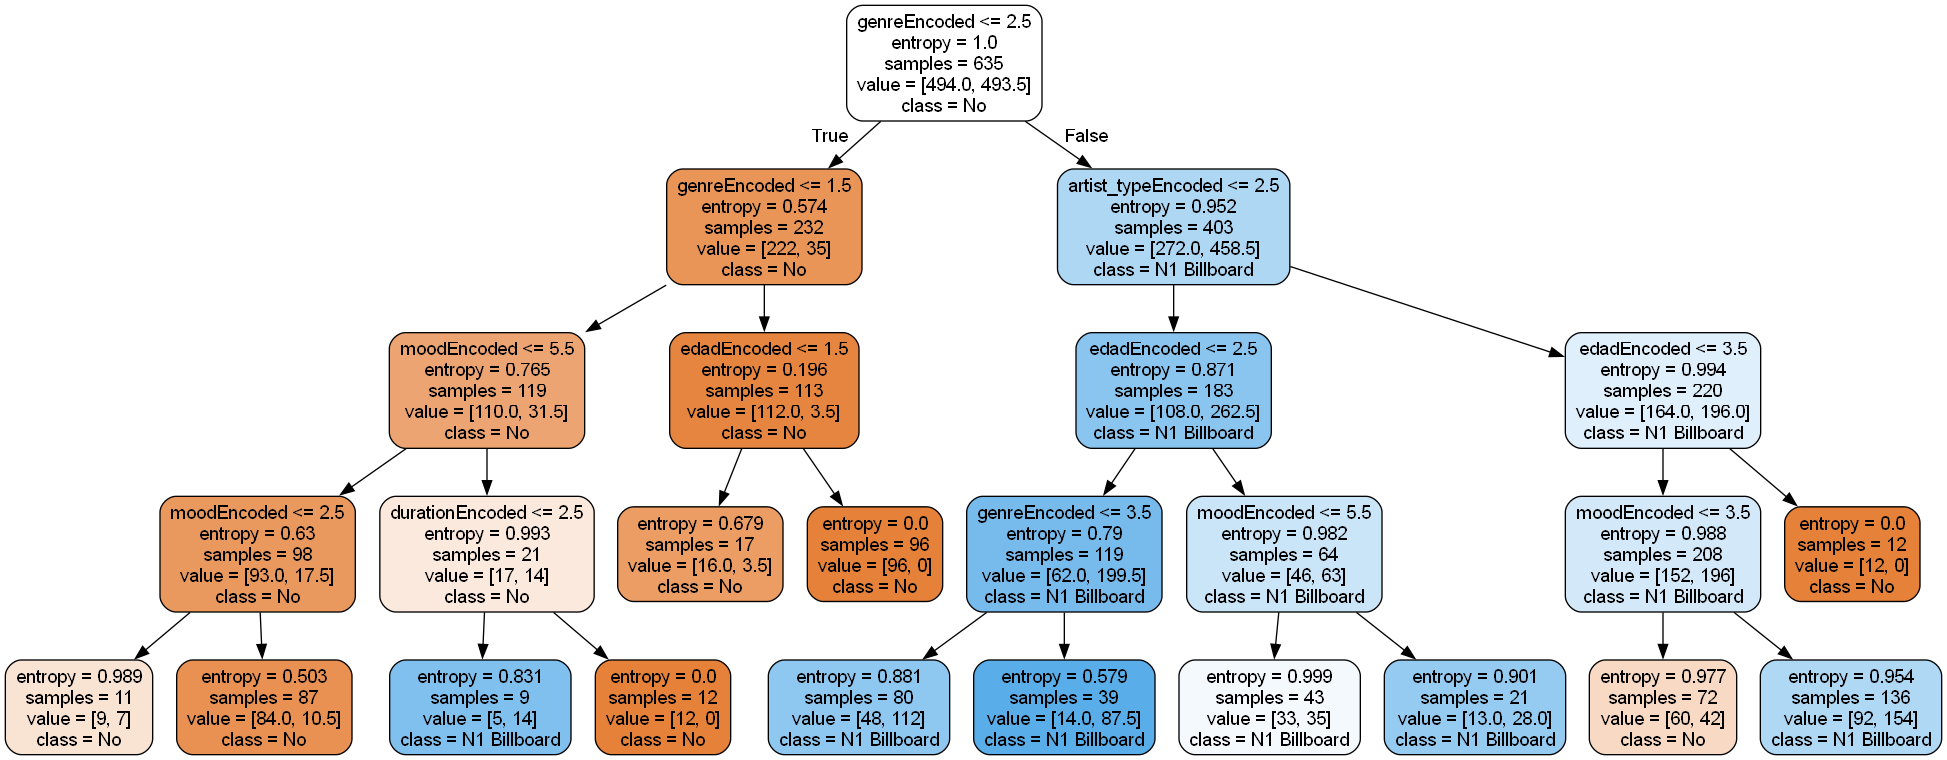
\includegraphics[width=1.2\textwidth]{tree1.png}
    \caption{{\small Árbol de Decisión }}
    \label{fig:enter-label}
\end{figure}



\textbf{Análisis}


\begin{figure}[H]
    \centering
\includegraphics[width=0.2\textwidth]{precision.png}
    \caption{{\small La precisión del árbol tiene un valor de 64.88\%. }}
    \label{fig:enter-label}
\end{figure}



\textbf{Predicción de Canciones al Billboard 100}


\begin{figure}[H]
    \centering
\includegraphics[width=0.3\textwidth]{p1.png}
    \caption{{\small Nos da que Havana llegará al top 1 con una probabilidad de 83\%. }}
    \label{fig:enter-label}
\end{figure}

\begin{figure}[H]
    \centering
\includegraphics[width=0.3\textwidth]{imagine.png}
    \caption{{\small La canción de Imagine Dragon NO llegará al top 1 con una certeza del 88\%. }}
    \label{fig:enter-label}
\end{figure}




\section{Conclusión}

El realizar esta actividad acerca de los árboles de decisión me permitió comprender su funcionamiento e utilidad para clasificar y predecir gran cantidad de datos, destacando la importancia de todo lo que se debe de realizar antes de crear el árbol de decisión (como analizar la coherencia de los datos con los que estamos trabajando y cambiarlos en caso de que haya algo ``raro'' en el conjunto de datos), la selección de profundidad y la interpretación de nodos. Pude ver la efectividad del árbol para identificar patrones en los datos y realizar predicciones claras y precisas. A parte de todo eso, el estar codificando me ayudó mucho en comprender el funcionamiento de varias funciones y métodos.



\section{Referencias}
Bagnato, J. (2020). Aprende Machine Learning en Español.


\end{document}
